\documentclass[10pt,a4paper]{article}
\usepackage[utf8]{inputenc}
\usepackage{amsmath}
\usepackage{amsfonts}
\usepackage{amssymb}
\usepackage{graphicx}
\usepackage{caption}
\usepackage[francais]{babel}

\begin{document}


\section{OpenMOLE}

\subsection{Le logiciel}

L'étude des systèmes complexes par la simulation numérique nécessite le traitement de gros volumes de données et l’exécution de calculs massifs. Cependant la mise en œuvre des méthodes numériques d'analyse avancées sur des environnements de calcul distribués s’avère très technique et loin des compétences des modélisateurs spécialistes de la thématique.

OpenMOLE\footnote{openmole.org} est un logiciel libre né de ce besoin fort: exécuter d'énormes quantités de calculs sur les modèles de systèmes complexes. Pour répondre à cette question, OpenMOLE permet: d’exécuter de très nombreuses instance des codes de calculs des utilisateurs (implémentés dans à peu près n'importe quel langage) grâce à du calcul distribué, d’exécuter des méthodes d'analyse numérique clef en main (algorithmes d'optimisation, de calibration, d'analyse de sensibilité…), de béneficier de maniére transparente de la puissance de calcul d'un large éventail d'environnements massivement parallèles  (serveurs multi-processeurs, fermes de calcul, grilles de calcul).


\section{Stratégie cloud}

OpenMOLE se présente sous forme d'un language dédié à l'exploration des modéles de simulation. Depuis, la version 5 (publiée début septembre), OpenMOLE propose une interface graphique qui guide l'utilisateur dans l'utilisation du logiciel. Cette avancé ergonomique a déjà permis l'adoption d'OpenMOLE 5 par plus de 50 utilisateurs en seulement 2 mois. 

\begin{figure}[h]
 \centering
  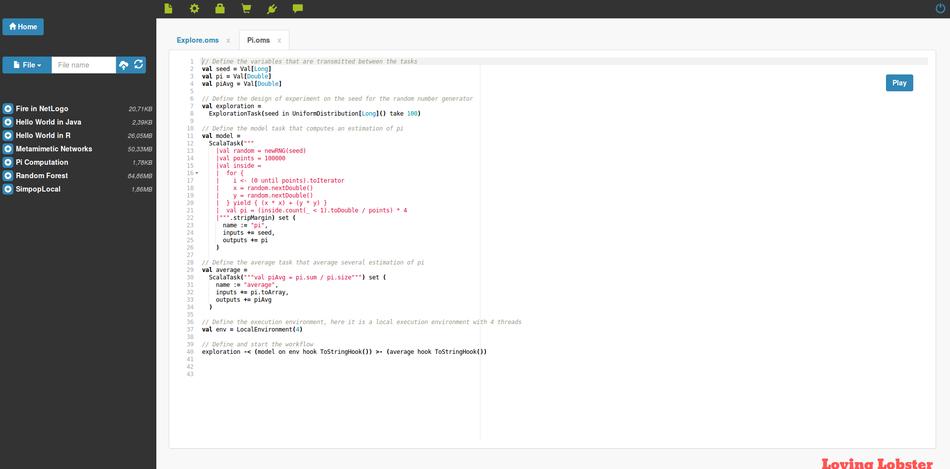
\includegraphics[width=0.8\linewidth]{img/openmoleUI.png}
 \captionof{figure}{ \label{UI} Capture d'écran de l'interface d'OpenMOLE}
\end{figure}

L'interface graphique représente une avancée importante dans l'utilisabilité d'OpenMOLE par des chercheurs de toutes disciplines. Cependant elle nécessite toujours une installation du logiciel sur la machine de l'utisateur. Cette opération pose deux problemes: d'une part elle confronte l'utilisateur à une opération technique qui peut s'avérer complexe et décourager l'utilisateur avant même qu'il puisse tester le logiciel. D'autre part, la machine sur laquelle est installée OpenMOLE doit rester allumée et connectée au réseau pendant tout le temps de l'execution de workflows qui peuvent pourtant durrer plusieurs jours.

Pour régler ce problème, nous développons actuellement une version d'OpenMOLE "dans les nuages". Grace à cette nouvelle fonctionnalité, les utilisateurs pourront se connecter via leur navigateurs web sur une instance distante d'OpenMOLE, qui leur permettra de développer et d'executer des workflows.

\section{Infrastructure}

Pour promouvoir OpenMOLE et rendre service à la communnauté l'ISC-PIF mettra à disposition 2 instances d'OpenMOLE. La premiére servira d'instance de démonstration. Elle permettra à des potentiels utilisateurs, souhaitant tester OpenMOLE, de le faire sans procédure d'inscription ou d'installation préalable. Cette instance propsera une version cloisonnée d'OpenMOLE servant à montrer ses fonctionnalités sans pour autant permettre de passer à l'échelle ou de faire persister des données. La deuxiéme instance mettra à disposition un service OpenMOLE complet. Cette instance nécessitera une inscription au service. Elle permettra de passer à l'échelle et de stocker des données de maniére péreine.

\begin{figure}[h]
 \centering
  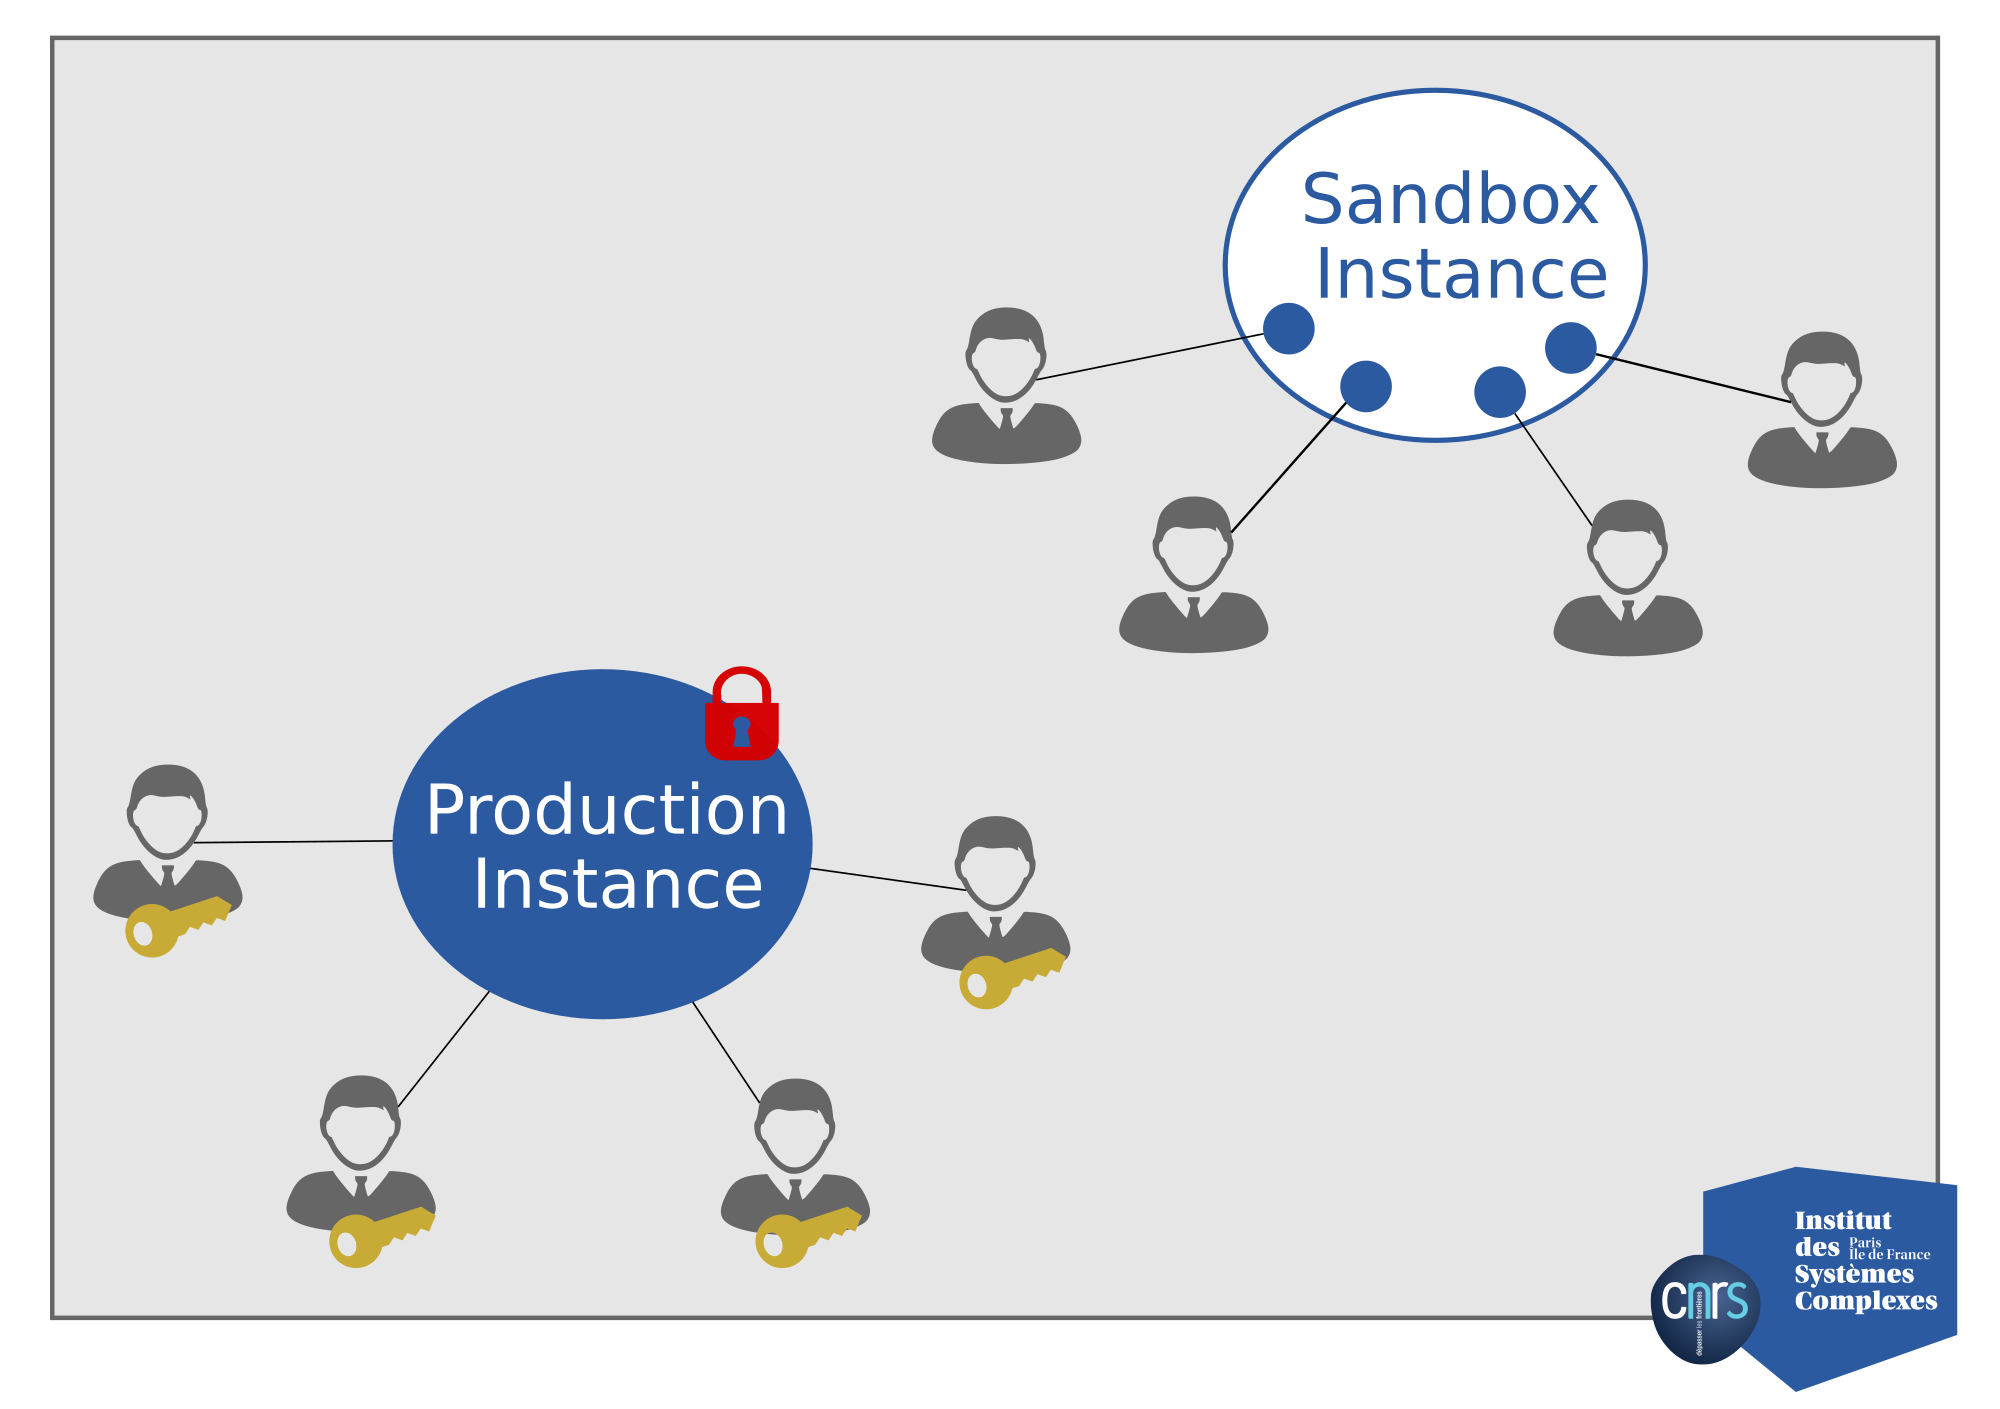
\includegraphics[width=0.8\linewidth]{img/instances.png}
 \captionof{figure}{ \label{service} Services OpenMOLE}
\end{figure}

\section{Passage à l'échelle}

En complément de l'instance central l'ISC-PIF formera les administrateurs systémes des laboratoires partenaires qui souhaitent déployer leur propre instance d'OpenMOLE. Tous les serveurs feront parti d'un réseau peer 2 peer qui permettra un échange facile des données et le travail collaboratif sur les workflows quelque soit le serveur depuis lequel l'utilisateur travaille.

\begin{figure}[h]
 \centering
  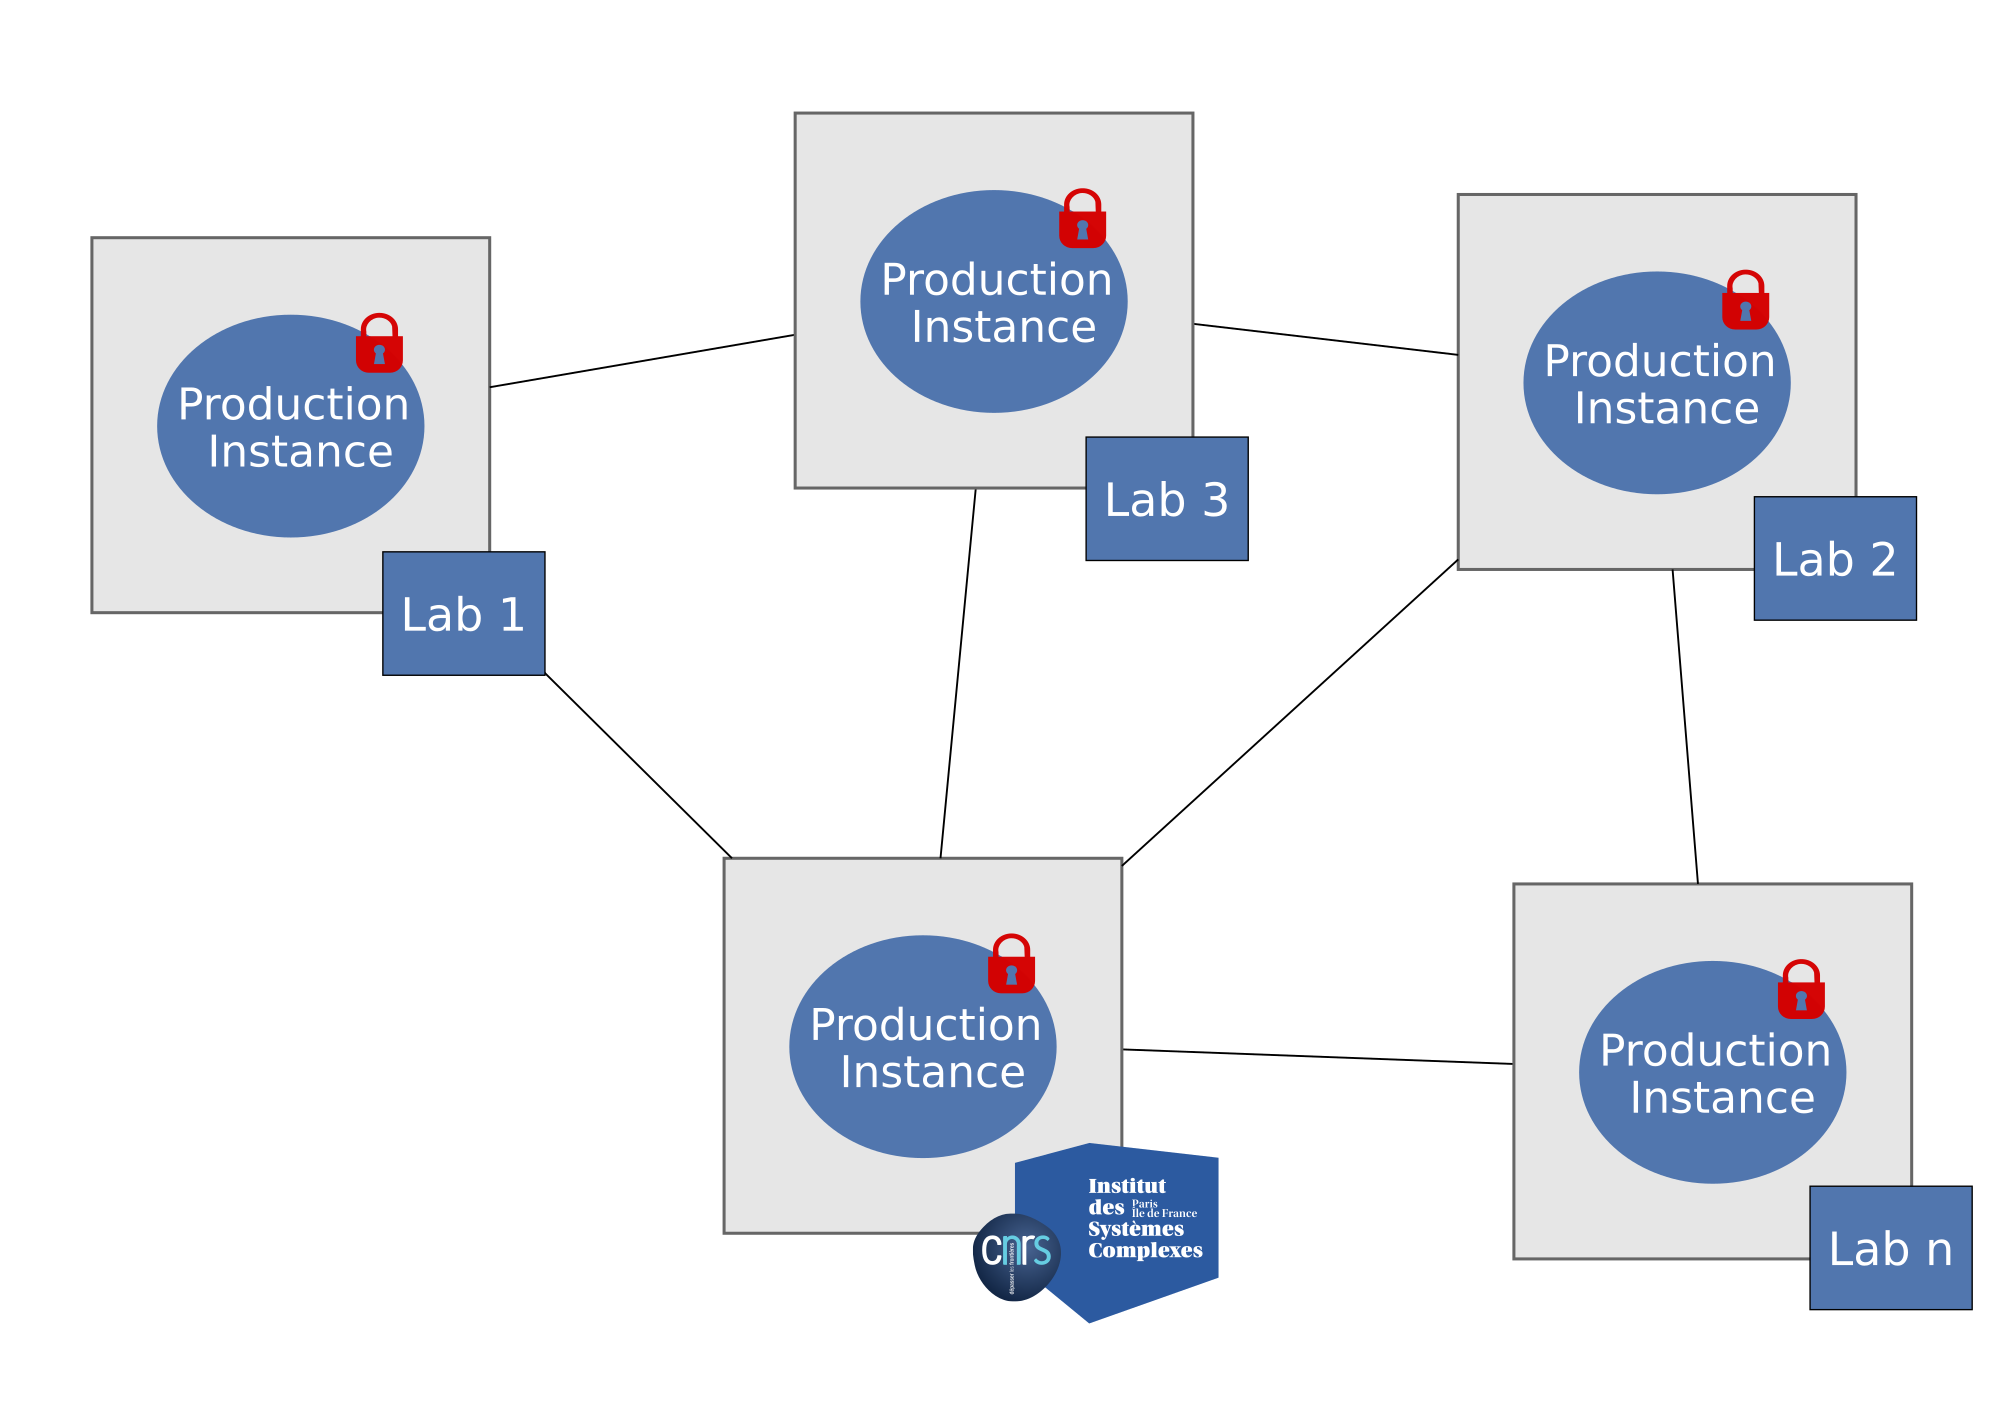
\includegraphics[width=0.8\linewidth]{img/instances-p2p.png}
 \captionof{figure}{ \label{reseau} Réseau OpenMOLE}
\end{figure}


\section{Besoins materiel}

Ressource par utilisateur sur le service de test : 1 coeur, 512 Mo de RAM, 1 Go de données.
Ressource par utilisateur sur le service de production : 1 coeur, 5 Go de RAM, 100 Go de données.

Capacité prévisionnelles : 10 utilisateurs simultané en test et 50 utilisateurs simultanés en productions.

Besoins matériel: 60 coeurs, 500 Go - 1 To de RAM, 10 To de disques.



\end{document}
